\begin{figure}[ht]
\begin{center}
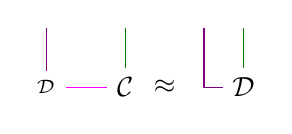
\begin{tikzpicture}[x=1cm,y=1cm]
  \node (sd1) at (0,1) {$\simul_{\mathcal{D}}$};
  \node (c1) at (1,1) {$\mathcal{C}$};
  \draw[color=Purple] (0,1.75) -- (sd1.north);
  \draw[color=Green] (1,1.75) -- (c1.north);
  \draw[color=Magenta] (sd1.east) -- (c1.west);
  \node (d1) at (2.5,1) {$\mathcal{D}$};
  \draw[color=Purple] (d1.west) -- (2,1) -- (2,1.75);
  \draw[color=Green] (d1.north) -- (2.5,1.75);
  \node at (1.5,1) {$\approx$};
\end{tikzpicture}
\end{center}
\caption{The second part of the precondition: $\mathcal{D}$ UC-emulates $\mathcal{C}$.}
\label{fig:commucbasicuc}
\end{figure}

%%% Local Variables:
%%% mode: latex
%%% TeX-master: "../main"
%%% End:
